\documentclass[11pt]{article}

\usepackage{pablo}
\usepackage{multicol}
\usepackage[a5paper,margin=1.2cm]{geometry}
\usetikzlibrary{calc}
\pagestyle{empty}

\begin{document}

\begin{center}
  \textsc{Devoir} --- Espace \& Probabilités

  Correction
\end{center}
\hrule

\begin{exercice}[Définitions]
  \begin{em}
  On lance un dé à 10 faces (numérotées de 1 à 10) équilibré, et on s'intéresse au nombre obtenu.
\end{em}
  \begin{enumerate}
    \item L'évènement «~Obtenir un nombre pair~» contient plusieurs issues (par exemple : « obtenir 2 » ; « obtenir 4 »). Ce n'est donc pas un évènement élémentaire.
    \item Le lancer étant équiprobable, la probabilité de «~Obtenir 9 ou 10~» est égale à $\frac{\text{Nombre d'issues favorables}}{\text{Nombre d'issues total}}=\frac{2}{10}=\frac{1}{5}$.
    \item
      \begin{enumerate}
        \item $P(\text{« Obtenir 1, 2, 3, 4 »}) = 0,4$.
      \item Une probabilité est un nombre compris entre 0 et 1 : elle ne peut pas être égale à 1,1.
    \end{enumerate}
    \item L'évènement « Obtenir 2 » est incompatible avec «~Obtenir un nombre impair~».
    \item Les issues correspondant à l'union des évènements «~Obtenir un multiple de 3~» et «~Obtenir un nombre supérieur à 7~» sont l'obtention de chacun des nombres 3, 6, 7, 8, 9, 10.
  \end{enumerate}
\end{exercice}

\begin{exercice}
  \emph{Soient $A$ et $B$ deux évènements tels que $P(A)=0,4$, $P(B)=0,2$, et $P(A\cap B)=0,1$.}
  \begin{enumerate}
    \item $\bar A$ est le contraire de $A$, donc $P(A)+P(\bar A)=1$. Ainsi, $0,4+P(\bar A)=1$, et $P(\bar A)=0,6$.
    \item On sait que $P(A)+P(B)=P(A\cap B)+P(A\cup B)$. Donc $0,4+0,2=0,1+P(A\cup B)$, et $P(A\cup B)=0,5$.
  \end{enumerate}
\end{exercice}

\begin{exercice}[Tableau]~
  \begin{multicols}{2}
  \begin{enumerate}
    \item Le tableau complété est ci-contre :
  \end{enumerate}

  \columnbreak

  \begin{center}
  \begin{tabular}{p{1.2cm}|p{0.8cm}|p{0.8cm}|p{0.9cm}}
  & N\up{o} 1 & N\up{o} 2 & Total \\
  \hline
  Blanche & 15\% & 30\% & 45\% \\
  \hline
  Noire   & 10\% & 45\% & 55\% \\
  \hline
  Total   & 25\% & 75\% & 100\%\\
\end{tabular}
\end{center}
\end{multicols}
\begin{enumerate}
    \setcounter{enumi}{1}
  \item $P(\text{« Obtenir une boule noire portant le numéro 2 »})=45\%$.
  \item $P(\text{«~Tirer une boule noire ou numérotée 2~»})=10\%+45\%+30\%=85\%$ : C'est somme des probabilités des évènements : « Tirer une boule noire numérotée 2 », « Tirer une boule noire numérotée 1 », et « Tirer une boule blanche numérotée 2 ».
  \item $P(\text{« Tirer une boule blanche numérotée 2 »})=30\%$
  \end{enumerate}
\end{exercice}

\begin{exercice}[Boule]\emph{Toutes les longueurs sont données en centimètres.}

  \begin{multicols}{2}
    \noindent On considère le parallélépipède rectangle $ABCDEFGH$ représenté ci-contre (la figure n'est pas à l'échelle), avec les longueurs $AB=6$, $BC=6$, $BF=3$.

  \begin{center}
  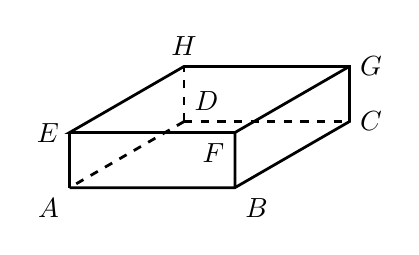
\begin{tikzpicture}[scale=0.7,line width=1pt]
    \coordinate (O) at (0,0);
    \coordinate (x) at (3,0);
    \coordinate (y) at ({3*0.8*cos(30)},{3*0.8*sin(30)});
    \coordinate (z) at (0,1);

    \coordinate (A) at (O);
    \coordinate (B) at ($(O) + (x)$);
    \coordinate (C) at ($(O) + (x) + (y)$);
    \coordinate (D) at ($(O) + (y)$);
    \coordinate (E) at ($(O) + (z)$);
    \coordinate (F) at ($(O) + (z) + (x)$);
    \coordinate (G) at ($(O) + (z) + (x) + (y)$);
    \coordinate (H) at ($(O) + (z) + (y)$);

    \draw (A) node[below left]{$A$};
    \draw (B) node[below right]{$B$};
    \draw (C) node[right]{$C$};
    \draw (D) node[above right]{$D$};
    \draw (E) node[left]{$E$};
    \draw (F) node[below left]{$F$};
    \draw (G) node[right]{$G$};
    \draw (H) node[above]{$H$};
    \draw (A) -- (B) -- (C) -- (G) -- (H) -- (E) -- (F) -- (B);
    \draw (A) -- (E);
    \draw (F) -- (G);
    \draw[dashed] (D) -- (H);
    \draw[dashed] (D) -- (A);
    \draw[dashed] (D) -- (C);
  \end{tikzpicture}

\end{center}
\end{multicols}

\begin{enumerate}
  \item \emph{Calculer la longueur du segment $[AC]$.} Le triangle $ABC$ est rectangle en $B$ (car $ABCD$ est un rectangle), donc on peut appliquer le théorème de Pythagore : $AB^2+BC^2=AC^2$. Donc $AC^2=6^2+6^2=72$, et $AC=\sqrt{72}$.
  \item \emph{En admettant que $ACG$ est rectangle en $C$, montrer que $AG=9$.} De même, on applique le théorème de Pythagore : $AG^2=AC^2+CG^2$, donc $AG^2=\sqrt{72}^2+3^2=72+9=81=9^2$, donc $AG=9$.
  \item \emph{En déduire le volume de la boule circonscrite à $ABCDEFGH$.} $AG$ étant le diamètre de la boule, son rayon est $AG/2$ soit $4,5$. Le volume d'une boule de rayon $r$ est donné par la formule $\frac{4}{3}\pi r^3$, donc le volume de la boule circonscrite est $\frac{4}{3}\pi\times4,5^3=\frac{3^5\pi}{2}\approx382~cm^3$.
\end{enumerate}
\end{exercice}

\begin{exercice}[Exercice ouvert]
  \begin{multicols}{2}
    \begin{em}
  \noindent On considère le cube $ABCDEFGH$, de côté 2~cm. Le point $I$ est le centre de la face $AEFB$ ; $J$ est le centre de la face $CGFB$. Quelle est la longueur du segment $[IJ]$ ?
\end{em}

  \begin{center}
  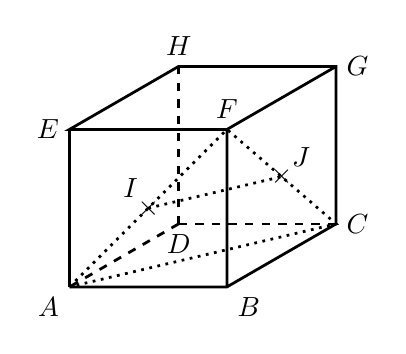
\begin{tikzpicture}[scale=2,line width=1pt]
    \coordinate (O) at (0,0);
    \coordinate (x) at (1,0);
    \coordinate (y) at ({0.8*cos(30)},{0.8*sin(30)});
    \coordinate (z) at (0,1);

    \coordinate (A) at (O);
    \coordinate (B) at ($(O) + (x)$);
    \coordinate (C) at ($(O) + (x) + (y)$);
    \coordinate (D) at ($(O) + (y)$);
    \coordinate (E) at ($(O) + (z)$);
    \coordinate (F) at ($(O) + (z) + (x)$);
    \coordinate (G) at ($(O) + (z) + (x) + (y)$);
    \coordinate (H) at ($(O) + (z) + (y)$);
    \coordinate (I) at ($(O) + 0.5*(x) + 0.5*(z)$);
    \coordinate (J) at ($(O) + (x) + 0.5*(y) + 0.5*(z)$);

    \draw (A) node[below left]{$A$};
    \draw (B) node[below right]{$B$};
    \draw (C) node[right]{$C$};
    \draw (D) node[below]{$D$};
    \draw (E) node[left]{$E$};
    \draw (F) node[above]{$F$};
    \draw (G) node[right]{$G$};
    \draw (H) node[above]{$H$};
    \draw (A) -- (B) -- (C) -- (G) -- (H) -- (E) -- (F) -- (B);
    \draw (A) -- (E);
    \draw (F) -- (G);
    \draw[dashed] (D) -- (H);
    \draw[dashed] (D) -- (A);
    \draw[dashed] (D) -- (C);

    %\draw[dotted] (A) -- (F) -- (C);
    \draw (I) node{$\times$} node[above left]{$I$};
    \draw (J) node{$\times$} node[above right]{$J$};
    \draw[dotted] (I) -- (J);
    \draw[dotted] (A) -- (F) -- (C) -- cycle;
  \end{tikzpicture}
\end{center}
\end{multicols}

Toutes les longueurs sont en centimètres.

Considérons le triangle $AFC$. Les points $I$ et $J$ sont respectivement les milieux des segments $[AF]$ et $[CF]$. D'après l'énoncé des milieux, la longueur $IJ$ est égale à la moitié de la longueur $AC$. Reste à calculer $AC$.

Le triangle $ABC$ est rectangle en $B$ (car $ABCD$ est un carré), donc on peut y appliquer le théorème de Pythagore : $AC^2=AB^2+BC^2=2^2+2^2=8$. Donc $AC=\sqrt{8}=2\sqrt{2}$.

Donc $IJ=\frac{AC}{2}=\frac{2\sqrt{2}}{2}=\sqrt{2}\approx1,4cm$.
\end{exercice}

\end{document}
